\documentclass[a4paper,10pt]{article}
\usepackage[utf8]{inputenc}
\usepackage{amsmath,amssymb,graphicx}
\usepackage{tikz}
\usepackage{xcolor}
\usepackage{hyperref}
\usepackage{listings}
\usepackage{geometry}
\geometry{margin=2cm}

\title{\textbf{Simulación: Partícula en Triángulo Equilátero}}
\author{Física Computacional}

\begin{document}
\maketitle

\begin{abstract}
Este proyecto simula el movimiento de una partícula confinada dentro de un triángulo equilátero con colisiones perfectamente elásticas. Se implementa en C++ con visualización mediante Gnuplot, demostrando el comportamiento dinámico de una partícula en un potencial infinito con geometría triangular.
\end{abstract}

\section{Introducción}
El estudio de partículas confinadas en regiones geométricas es fundamental en física estadística y mecánica clásica. En este trabajo se analiza el caso particular de un triángulo equilátero, donde la partícula experimenta colisiones elásticas perfectas con los bordes.

\section{Marco Teórico}

\subsection{Geometría del Triángulo Equilátero}
Para un triángulo de lado $L$, las coordenadas de los vértices son:
\begin{align*}
A &= (0, 0) \\
B &= (L, 0) \\
C &= \left(\frac{L}{2}, \frac{\sqrt{3}}{2}L\right)
\end{align*}

\subsection{Ecuaciones de los Lados}
\begin{itemize}
\item \textbf{Base (AB)}: $y = 0$
\item \textbf{Lado izquierdo (AC)}: $y = \sqrt{3}x$
\item \textbf{Lado derecho (BC)}: $y = -\sqrt{3}(x - L)$
\end{itemize}

\subsection{Condición de Interior}
Un punto $(x, y)$ está dentro del triángulo si:
\begin{align*}
y &\geq 0 \\
y &\leq \sqrt{3}x \\
y &\leq -\sqrt{3}(x - L) \\
y &\leq \frac{\sqrt{3}}{2}L
\end{align*}

\section{Modelo Físico}

\subsection{Colisiones Elásticas}
\begin{itemize}
\item \textbf{Conservación de energía}: $K = \frac{1}{2}m(v_x^2 + v_y^2)$ = constante
\item \textbf{Reflexión especular}: $\vec{v}' = \vec{v} - 2(\vec{v} \cdot \hat{n})\hat{n}$
\item \textbf{Vectores normales}:
  \begin{itemize}
  \item Base: $\hat{n} = (0, -1)$
  \item Lado izquierdo: $\hat{n} = (-\frac{\sqrt{3}}{2}, \frac{1}{2})$
  \item Lado derecho: $\hat{n} = (\frac{\sqrt{3}}{2}, \frac{1}{2})$
  \end{itemize}
\end{itemize}

\section{Implementación}

\subsection{Estructura del Proyecto}

\subsection{Algoritmo Numérico}
\begin{itemize}
\item \textbf{Método}: Integración Euler explícito
\item \textbf{Detección de colisiones}: Verificación analítica de bordes
\item \textbf{Actualización de velocidades}: Reflexión elástica con normales
\item \textbf{Paso temporal}: $\Delta t$ configurable por usuario
\end{itemize}

\section{Visualización}

\subsection{Gráficas Generadas}
\begin{itemize}
\item \textbf{Trayectoria 2D}: Movimiento en el plano $xy$
\item \textbf{Posición vs Tiempo}: $x(t)$ y $y(t)$ por separado
\item \textbf{Velocidades}: $v_x(t)$ y $v_y(t)$
\item \textbf{Animación}: Evolución temporal en formato GIF
\end{itemize}

\begin{figure}[h]
\centering
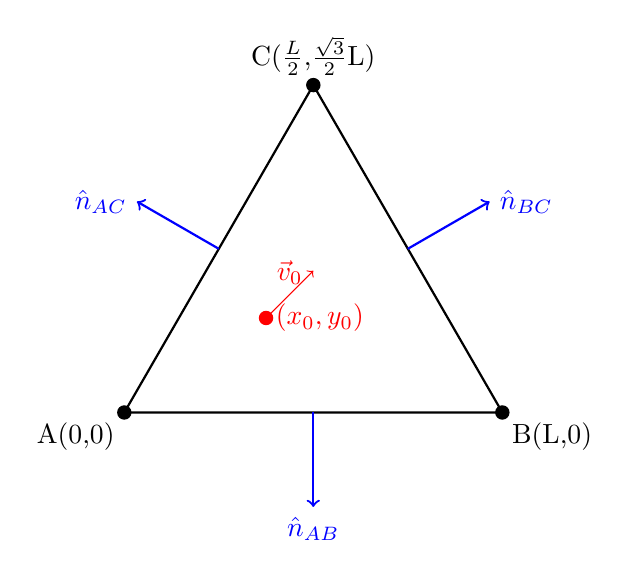
\begin{tikzpicture}[scale=1.2]
% Triángulo equilátero
\coordinate (A) at (0,0);
\coordinate (B) at (4,0);
\coordinate (C) at (2,3.464);

\draw[thick] (A) -- (B) -- (C) -- cycle;

% Vértices
\filldraw (A) circle (2pt) node[below left] {A(0,0)};
\filldraw (B) circle (2pt) node[below right] {B(L,0)};
\filldraw (C) circle (2pt) node[above] {C($\frac{L}{2}$,$\frac{\sqrt{3}}{2}$L)};

% Punto interior y trayectoria
\filldraw[red] (1.5,1) circle (2pt) node[right] {$(x_0,y_0)$};
\draw[red, ->] (1.5,1) -- (2.0,1.5) node[midway, above] {$\vec{v}_0$};

% Normales
\draw[blue, ->, thick] (2,0) -- (2,-1) node[below] {$\hat{n}_{AB}$};
\draw[blue, ->, thick] (1,1.732) -- (0.134,2.232) node[left] {$\hat{n}_{AC}$};
\draw[blue, ->, thick] (3,1.732) -- (3.866,2.232) node[right] {$\hat{n}_{BC}$};
\end{tikzpicture}
\caption{Geometría del triángulo equilátero con vectores normales en cada lado.}
\end{figure}

\section{Compilación y Uso}

\subsection{Requisitos}
\begin{itemize}
\item Compilador C++ (g++)
\item Gnuplot
\item Sistema Linux/Unix
\end{itemize}

\subsection{Ejecución}
\begin{verbatim}
$ make
$ ./bin/triangulo
\end{verbatim}

\subsection{Ejemplo de Entrada}
\begin{verbatim}
Lado del triángulo L (m): 10.0
Posición inicial x0 (m): 3.0
Posición inicial y0 (m): 2.0
Velocidad inicial vx0 (m/s): 2.0
Velocidad inicial vy0 (m/s): 1.5
Tiempo final tf (s): 20.0
Paso dt (s): 0.01
\end{verbatim}

\section{Análisis Físico}

\subsection{Propiedades Dinámicas}
\begin{itemize}
\item \textbf{Conservación de energía}: Verificada numéricamente
\item \textbf{Periodicidad}: Trayectorias pueden ser periódicas o caóticas
\item \textbf{Dependencia sensitiva}: Pequeños cambios en condiciones iniciales pueden llevar a comportamientos muy diferentes
\end{itemize}

\subsection{Validación}
\begin{itemize}
\item La partícula nunca escapa del triángulo
\item La energía cinética se mantiene constante
\item Los ángulos de incidencia y reflexión son iguales
\end{itemize}

\section{Resultados y Aplicaciones}

\subsection{Comportamientos Observados}
\begin{itemize}
\item \textbf{Trayectorias periódicas}: Para ciertas condiciones iniciales
\item \textbf{Comportamiento caótico}: Para la mayoría de condiciones
\item \textbf{Cobertura ergódica}: La partícula visita toda la región con el tiempo
\end{itemize}

\subsection{Aplicaciones}
\begin{itemize}
\item Estudios de billares dinámicos
\item Mecánica estadística de sistemas confinados
\item Simulación de gases en cavidades
\item Análisis de sistemas caóticos
\end{itemize}

\section{Conclusión}

Esta simulación proporciona una herramienta educativa para estudiar dinámicas de partículas en regiones confinadas con geometrías no triviales. El triángulo equilátero presenta propiedades interesantes debido a su simetría y ángulos agudos, generando comportamientos dinámicos ricos y complejos.


\end{document}